\chapter{Implementation}
\label{cha:Implementation}

\section{Generalising}
\label{sec:Generalising}

\begin{figure}[htb]
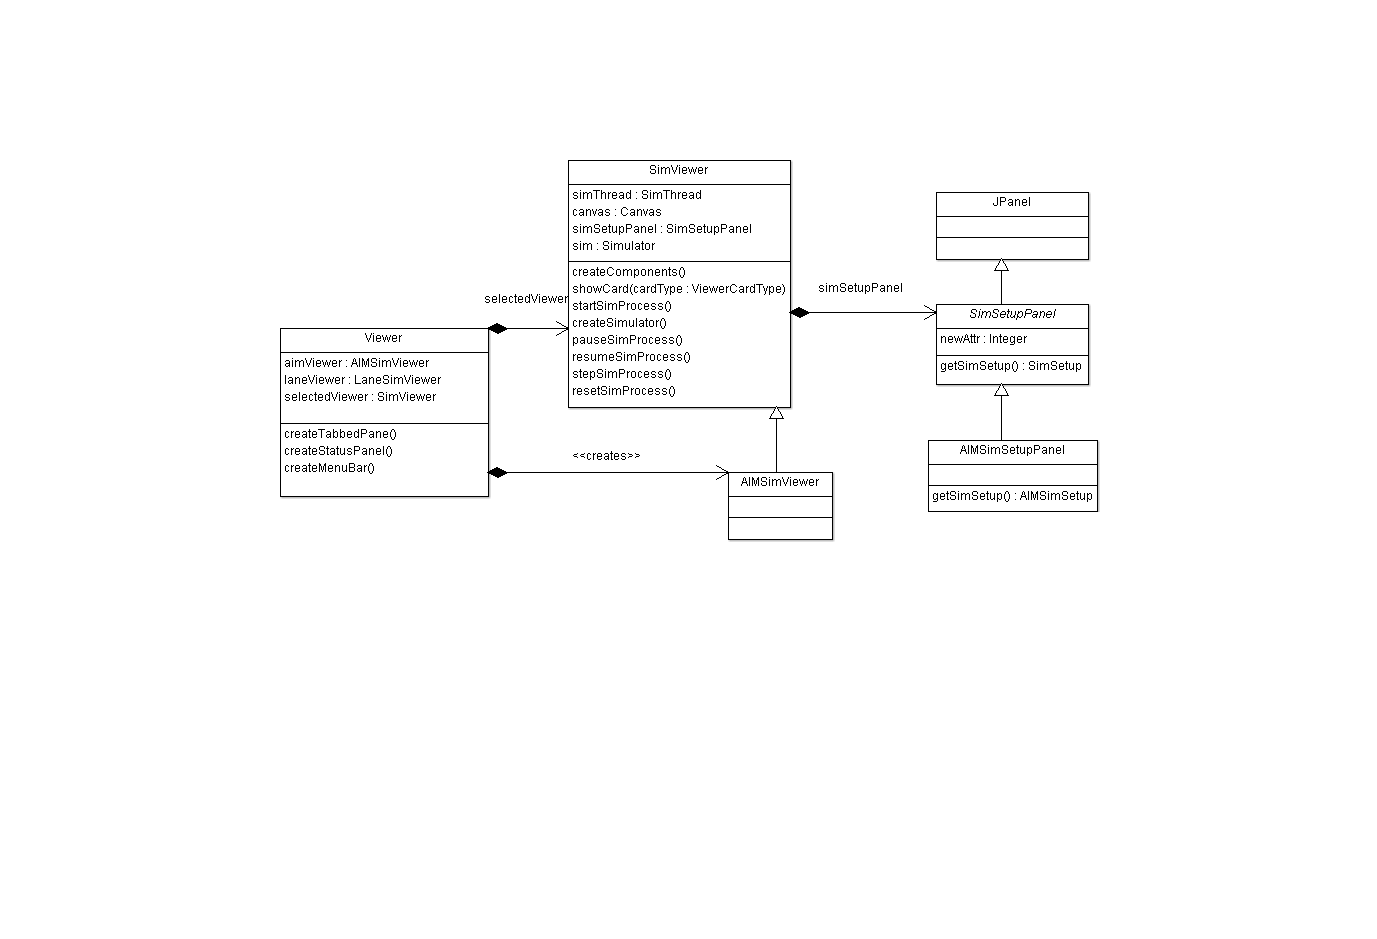
\includegraphics[width=\textwidth]{ViewerStructure.png}
\caption{Changes made to Viewer structure. Created SimViewer class to contain all GUI elements related to SimSetupPanel and Canvas. Subclasses of this deal with their own simulators separately.}
\end{figure}

\begin{figure}[htb]
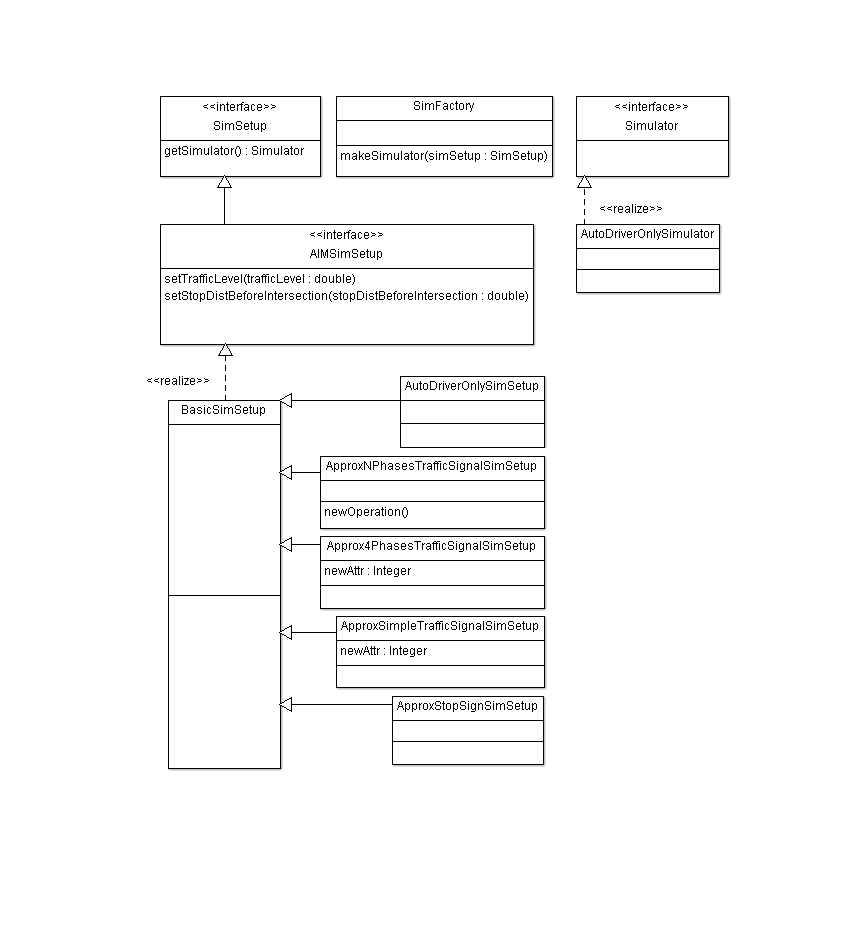
\includegraphics[width=\textwidth]{SimStructure.png}
\caption{Changes to Sim structure. SimSetup is now generalised. Only job is to produce a simulator object when called by SimFactory.}
\end{figure}